\section{User Centered Design} % (fold)
\label{sec:user_centered_design}

\HG aims to be helpful and usable for two specific target groups: history teachers and students in schools. The root problem we defined is that history is considered as boring and not interesting by a large portion of the students. One of the reasons we identified is that there exist not a lot of interesting and modern teaching material for teachers. We want to tackle this problem and develop a solution to help teachers presenting content of the history lessons in an interesting, informative and interactive way and for students to understand events and their coherences in history better.

We found a school in Jena, 25 km east of Weimar, that served as a development partner for the project, an instance of \HG directly designed for the usage in class.

\begin{figure}[H]
  \centering
  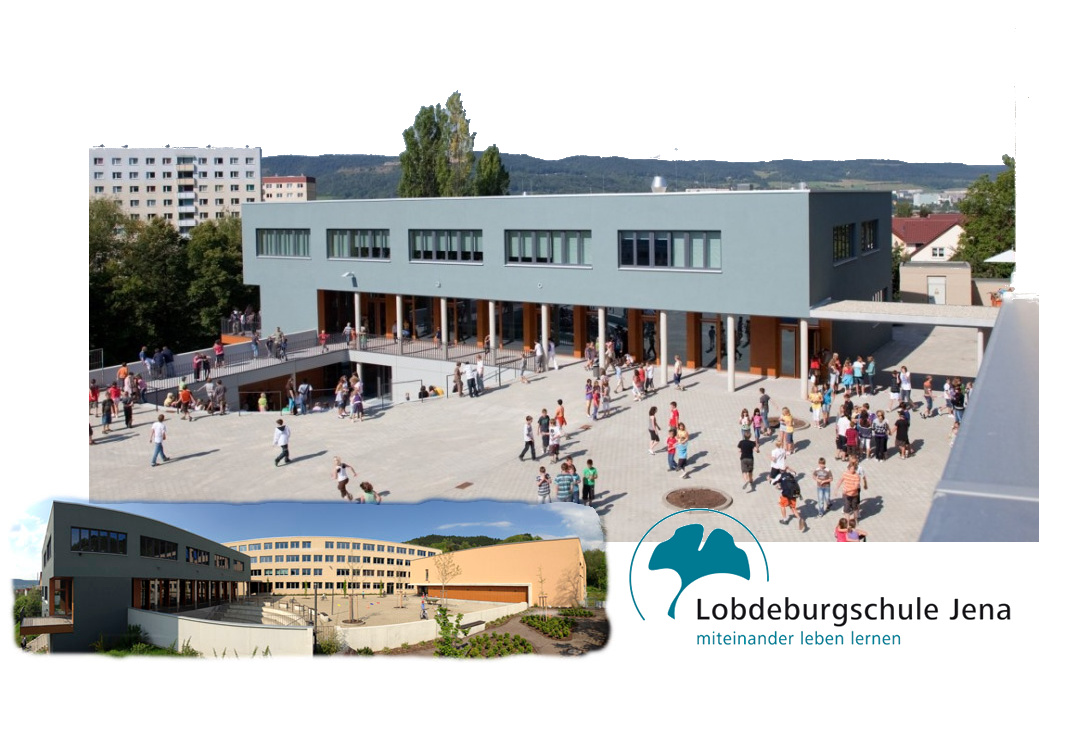
\includegraphics[width=0.9\textwidth]{graphics/lobdeburgschule.jpg}
\end{figure}

\paragraph{Lobdeburgschule} in Jena-Lobeda is a public school for all students from grade 1 to 13. A history teacher in grade 12 invited us to conduct a field study in his class to test \HG directly in school by the end of the project in April 2015. In the time period from October 2014 until the test in April 2015 two members of the project group went every two or three weeks to the teacher in Jena. We presented new concepts, asked specific questions about the interface and the usage of the visualization in class and new problems and questions about the concept raised that had to be clarified until the next meeting.

\begin{figure}[H]
  \centering
  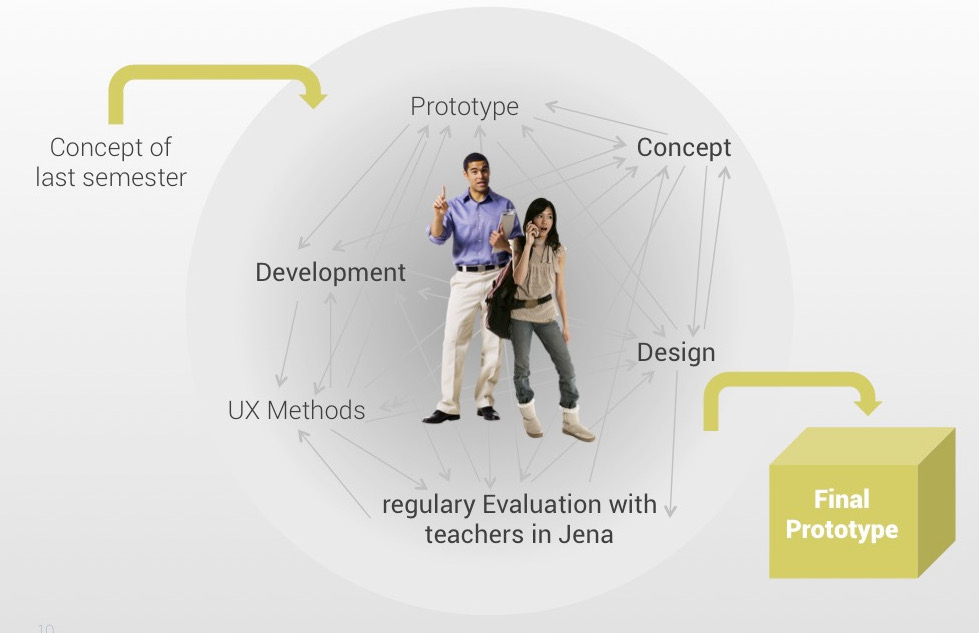
\includegraphics[width=0.7\textwidth]{graphics/design-1.jpg}
  \caption{User Centered Design}
\end{figure}

\paragraph{Design Iterations}
Through the project time a lot of different design concepts were developed. On the one hand we wanted to maximize the utility for the teacher to help him convey the necessary information in class but on the other hand design \HG in a way that we found suitable. We played around with the orientation and the functionality of the Timeline, the information about historical events on the map or the colors of the interface.

\begin{figure}[H]
  \centering
  \begin{minipage}{0.32\textwidth}
    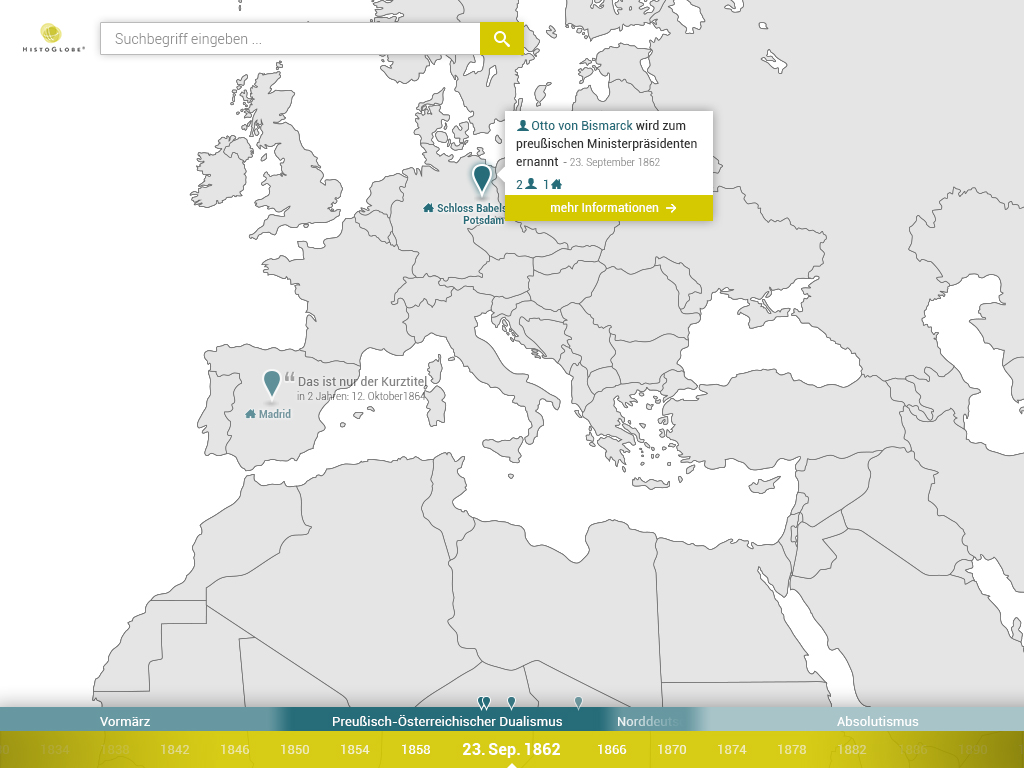
\includegraphics[width=0.95\textwidth]{graphics/design-2.jpg}
  \end{minipage}
  \begin{minipage}{0.32\textwidth}
    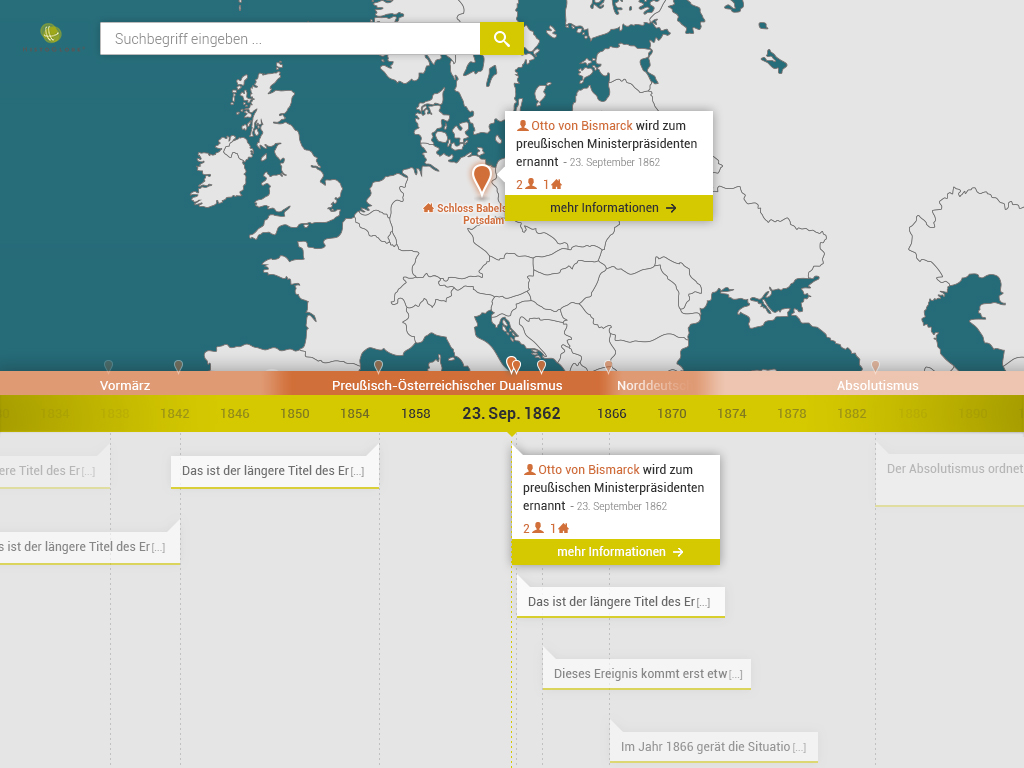
\includegraphics[width=0.95\textwidth]{graphics/design-3.jpg}
  \end{minipage}
  \begin{minipage}{0.32\textwidth}
    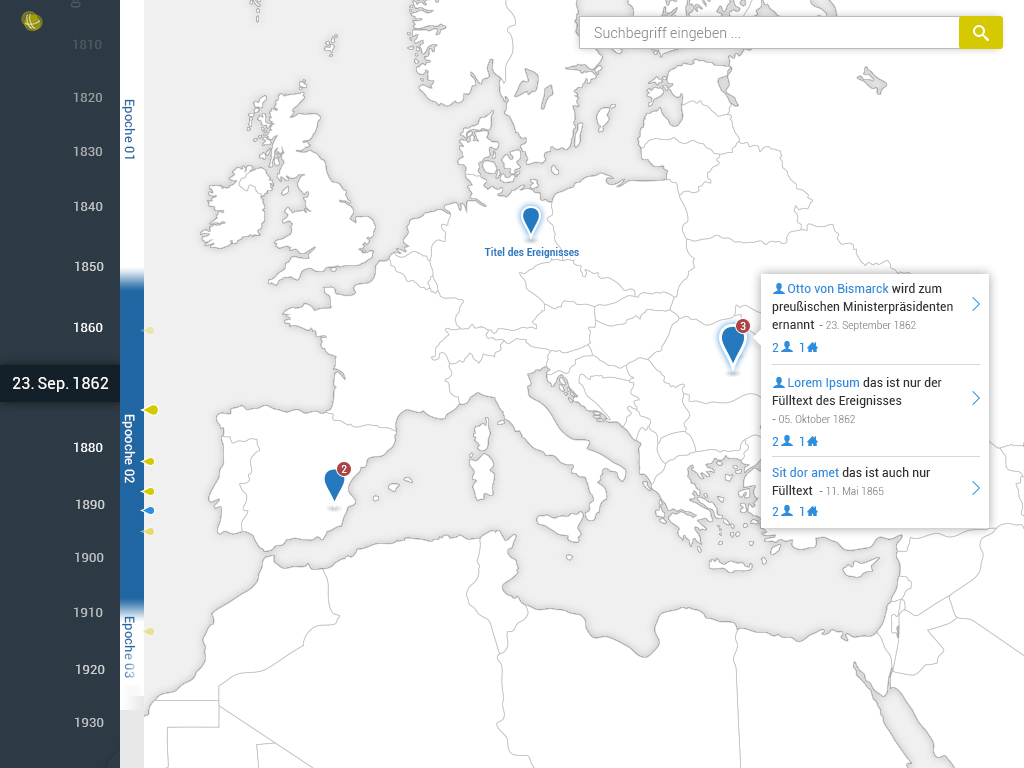
\includegraphics[width=0.95\textwidth]{graphics/design-4.jpg}
  \end{minipage}
  \caption{Several concepts of the design throughout the semester}
\end{figure}

In the next chapter we want to introduce the final elements of the user interface that were the result of the design iterations with the teacher.

% section user_centered_design (end)
